%=======================================================================
% Template para dissertação 
% Programa de Pós Graduação em Informática Aplicada da Universidade Federal 
% Rural de Pernambuco
%=======================================================================

%para incluir um arquivo por vez use \includeonly. 
%exemplos:
%\includeonly{capitulos/introducao,capitulos/bibliografia}
%\includeonly{capitulos/introducao,capitulos/conclusoes,capitulos/bibliografia}
%\includeonly{prefacios/capa2,prefacios/folha_rosto,prefacios/resumo,prefacios/abstract,capitulos/introducao,capitulos/bibliografia }

\documentclass [12pt,fleqn,oneside]{book}    % nomes e hifenação em português
\usepackage[brazil]{babel}         % Pacotes relativos à linguagem de entrada
\usepackage [utf8]{inputenc}     % aceitar texto acentuado em UTF-8
\usepackage {fancyhdr}             % cabeçalhos mais sofisticados
\usepackage {indentfirst}          % indentar 1a linha de cada seção

% Pacotes adicionados por mim
\usepackage{float}
\usepackage{nomencl}
\usepackage{multirow}
\usepackage{caption}
\usepackage{array}
\usepackage{tabularx}

% Pacotes relativos à inclusão de figuras
\usepackage {graphicx}         % para incluir figuras em PostScript
\usepackage{amsfonts,amsthm,amsopn,amssymb,latexsym}
\usepackage{geometry}
\usepackage[intlimits]{amsmath}
\usepackage{hyperref}
\usepackage{color}

% Dimensões da página
\usepackage{a4}                       % tamanho da página
\setlength{\textwidth}{16.5cm}        % largura do texto
\setlength{\textheight}{9.5in}        % tamanho do texto (sem head, etc)
\renewcommand{\baselinestretch}{1.4}  % espaçamento entre linhas
\addtolength{\topmargin}{-1cm}        % espaço entre o head e a margem
\setlength{\oddsidemargin}{-0.1cm}    % espaço entre o texto e a margem
\setlength{\parindent}{.0in}          % identação na 1a linha de cada parágrafo
\sloppy                               % Ser indulgente no preenchimento das linhas
\parskip 10pt                         % Espaçamento entre parágrafos

%alguns macros
\newtheorem{teo}{Teorema}[chapter]
\newtheorem{lema}[teo]{Lema}
\newtheorem{cor}[teo]{Corol\'{a}rio}
\newtheorem{prop}[teo]{Proposi\c{c}\~{a}o}
\newtheorem{defin}[teo]{Defini\c{c}\~ao}
\newtheorem{Af}[teo]{Afirma\c{c}\~{a}o}
\newtheorem{ex}[teo]{Exemplo}
\newtheorem{obs}[teo]{Observa\c{c}\~{a}o}
\newcommand{\R}{\ensuremath{\mathbb{R}}}
\newcommand{\Rn}{{\ensuremath{\mathbb{R}}}^{n}}
\newcommand{\Rm}{{\ensuremath{\mathbb{R}}}^{m}}
\newcommand{\Rnn}{{\ensuremath{\mathbb{R}}}^{ n \times n }}
\newcommand{\N}{\ensuremath{\mathbb{N}}}
\newcommand{\Z}{\ensuremath{\mathbb{Z}}}
\newcommand{\blackbox}{\rule{2mm}{2mm}}
\newcommand{\raiz}{\mbox{raiz}}
\newcommand{\contcaption}[1]{\vspace*{-0.1\baselineskip}\begin{center}#1\end{center}\vspace*{0.3\baselineskip}}

% Definindo as barras para a capa
\newcommand{\HRule}{\rule{\linewidth}{1mm}}

% Customização da Lista de Siglas
\makenomenclature
\renewcommand{\nomname}{Lista de Siglas}

% ====================================================================================


% Início do texto
\begin {document}

% Páginas sem numeração (capa, agradecimentos, etc)
\pagestyle {empty}

% Páginas iniciais
\begin{figure}[h]
\leavevmode
\begin{minipage}{\textwidth}

\includegraphics[scale=0.7]
{prefacios/capa/logo-ufrpe.eps}
\end{minipage}
\end{figure}
\vspace{-3.5cm}
{\bf
\begin{center}
{\Large
\hspace*{0cm}Universidade Federal Rural de Pernambuco \\
\hspace*{0cm}Departamento de Estatística e Informática}\\
\end{center}
}
\noindent
\begin{figure}[h]
\centering

\includegraphics[scale=0.5]{prefacios/capa/logo-bsi-presencial-v3-amp.eps}
\end{figure}


\vspace{2.5cm}
\noindent
\begin{center}
{\Large \bf Um Estudo sobre Lições Aprendidas na Adoção de Métodos Ágeis por Organizações de Software} \\[5cm]
{\Large Daniel Filype Silva Barreto}\\[6mm]
\end{center}


\vspace{1.5cm}
\begin{center}
{\large {\bf Recife}\\[6mm]
Março de 2014}
\end{center}
\newpage
           % capa ilustrativa
%
\hyphenation{}

\vspace*{0.0cm}
{\center
{\Large Daniel Filype Silva Barreto}\\[2.4cm]
{\huge \bf Um Estudo sobre Lições Aprendidas na Adoção de Métodos Ágeis por Organizações de Software}\\[2.0cm]
{\Large Orientador: Teresa Maciel}}\\[2.0cm]

{\raggedleft
\begin{minipage}[t]{8.3cm}
\setlength{\baselineskip}{0.25in}
Monografia apresentada ao Curso Bacharelado em Sistemas de Informação  da Universidade Federal Rural de Pernambuco, como requisito parcial para obtenção do título de Bacharel em Sistemas de Informação.\end{minipage}\\[2cm]}
\vspace{3cm}
{\center Recife \\[3mm]
Março de 2014 \\}

\newpage
\vspace*{18cm}
{\raggedleft
\begin{minipage}[t]{6.0cm}
\setlength{\baselineskip}{0.25in}
À minha mãe, Izabel\\
À minha namorada, Bruna\\
À minha orientadora, Teresa\\
Aos meus amigos\\
\end{minipage}\\[2cm]}



\newpage
\begin{center}
{\Large \bf Agradecimentos}
\end{center}
\vspace*{-0.06in}

À minha mãe, Izabel, que desde pequeno me mostrou o quanto a busca por conhecimento é importante.

À minha namorada, Bruna, por sempre estar ao meu lado em todos os momentos importantes da minha vida.

À minha orientadora, Teresa, que sempre esteve disponível e disposta a me ajudar.

Aos meus amigos de infância que, mesmo indiretamente, incentivaram-me a seguir em frente.


     % capa ABNT

% Numeração em romanos para páginas iniciais (sumários, listas, etc)
\pagenumbering {roman}
\pagestyle {plain}

% Geração do sumário, agradecimentos, e etc..
\chapter*{Resumo}
escreva o resumo do trabalho...

         % resumo em português
\chapter*{Abstract}

Agile development methodologies aim to build software in a faster and more efficient way, creating a minimum product that already brings value to the customer and, thenceforth, adding new features to it. This is a complete paradigm shift if we compare them with the planning-driven methodologies.

Changing drastically is never easy. Given this scenario, a research line focused on the study of this transition process from planning-driven methodologies to Agile has emerged. According to its studies, the main benefits from the adoption of agile methods are: customer satisfaction, more frequent deliveries, maintainability of the team morale high, improvement on the quality of the final product and so on. However, conquering all these benefits requires a lot of discipline and dedication.

Analyzing the results obtained with this research, a more common set of lessons learned was perceived. Among them, we can cite: ``customization and adaptability", ``experience, training and learning", ``engagement, commitment, discipline and teamwork" and ``technical and technological aspects".

\textbf{Keywords:} Agile methods, agile adoption, lessons learned

\tableofcontents                    % sumário
\listoftables                       % lista de tabelas
\listoffigures                      % lista de figuras
\printnomenclature		     % lista de siglas
%\listofprograms                    % lista de programas
\clearpage


%=======================================================================
% Definir um estilo para páginas completas (cabeçalho + rodapé)
\pagestyle {fancyplain}

% Marca de capítulo do tipo "2. Blábláblá..." no cabeçalho
\renewcommand{\chaptermark}[1]{\markboth{\thechapter.\ {#1}}{}}

% Para aumentar o tamanho da caixa para o cabeçalho
\addtolength{\headheight}{\baselineskip}

% Definindo o conteúdo do cabeçalho...
\fancyhf{}
\fancyhead[L,L]{\nouppercase{\textsf{\leftmark}}} %comentar
\fancyhead[R,R]{\thepage}

% Para garantir que a primeira página de cada capítulo...
\fancypagestyle{plain}{
\fancyhf{}                          % não terá head ou foot
\renewcommand{\headrulewidth}{0pt}} % nem linhas de cabeçalho
%=======================================================================


% Capítulos são numerados em algarismos arábicos
\setcounter{page}{0} \pagenumbering{arabic}

%incluir os arquivos dos capítulos
% Os arquivos de cada capítulo devem iniciar com \chapter{Nome do Capítulo}
% (o nome deve terminar com .tex)
\chapter{Introdução}

\section{Apresentação}

O Manifesto Ágil \cite{agileManifesto}, criado em 2001, revolucionou o mercado de Tecnologia da Informação, pois, até então, a maneira de se desenvolver software mostrou-se falha em diversos aspectos. Contudo, a transição entre os modelos antigos (conhecidos como “plan-driven”) e o moderno (conhecido como Ágil) é uma tarefa não-trivial.

As principais motivações por trás da adoção ágil de desenvolvimento de software são: a melhoria da qualidade do produto final, aumento da moral dos desenvolvedores e satisfação do cliente. Entretanto, adoção ágil sempre vem com desafios especiais e, para que ela ocorra com sucesso, mudanças fundamentais na cultura da organização são necessárias \cite{Hajjdiab2011}. Este projeto visa expor lições aprendidas por empresas de desenvolvimento de software que passaram por este processo.

\section{Justificativas}

Muitas abordagens diferentes podem ser aplicadas a desenvolvimento de software \cite{Kettunen2010}, cada uma com suas peculiaridades. De acordo com \cite{Shore2007}, metodologias denominadas ágeis tornaram-se bastante populares, sendo utilizadas por grandes corporações como: Google, Yahoo!, Symantec, Microsoft, etc. Entretanto, não existe bala de prata no que tange a desenvolvimento de software. Não se deve simplesmente aplicá-las porque são populares. Existem vários estudos na literatura que mostram casos falhos de adoção de métodos ágeis \cite{Krasteva2008}. É preciso entender a fundo estas novas metodologias, analisar seus pontos positivos e negativos e, principalmente, refletir se elas agregariam valor ao produto final a ser entregue.

Sendo assim, é de suma importância a coleta de experiências para que se possa aprender sobre esta transição com aqueles que já passaram por este processo e que, além disso, querem contribuir com a comunidade de desenvolvimento de software.

\section{Objetivos} 

\subsubsection{Objetivo Geral}

\begin{itemize}
	\item Disponibilizar para acesso da indústria e academia de software um conjunto de lições aprendidas mais relatadas com a adoção de desenvolvimento ágil por organizações de software.
\end{itemize}

\subsubsection{Objetivos Específicos}

\begin{itemize}
	\item Investigar, através de pesquisa exploratória, a necessidade e contribuição de trabalhos desta natureza.
	\item Adquirir conhecimento sobre fundamentos teóricos relacionados como desenvolvimento ágil de software e lean.
	\item Realizar uma revisão utilizando como base a metodologia de revisão sistemática \cite{Barbara04} para coletar lições aprendidas provenientes de trabalhos publicados pela comunidade científica.
	\item Realizar uma pesquisa exploratória para coletar lições aprendidas provenientes de trabalhos publicados pela indústria de software nas principais conferências neste contexto.
	\item Identificar um conjunto de benefícios e desafios mais citados a partir dos resultados das pesquisas realizadas.
	\item Validar o trabalho realizado através de uma metodologia de survey \cite{Babbie1990}, aplicando-se questionários com profissionais brasileiros reconhecidos na área, assim como em empresas que adotam o desenvolvimento ágil.
	\item Gerar um protótipo de um banco de dados de lições aprendidas para acesso livre pela comunidade de software.
\end{itemize}

\section{Contribuições obtidas}

Com este trabalho, foi possível criar uma fonte única de informações relacionadas a processos de adoção ágil em empresas de desenvolvimento de software. Além disso, foi possível iniciar da criação de um protótipo de banco de dados de lições aprendidas que, dependendo do interesse da comunidade, pode vir a se tornar uma grande ferramenta colaborativa.

\section{Organização do trabalho}

Este trabalho é composto por mais três capítulos. No capítulo 2 está exposto o método utilizado para revisar a Literatura, juntamente com o conjunto de artigos científicos e relatos de experiência selecionados. No capítulo 3 encontra-se o resultado do mapeamento das lições aprendidas relatadas pelos trabalhos selecionados. O capítulo 4 apresenta a validação do que foi construído com o projeto (através de um questionário), suas conclusões e possíveis futuros trabalhos.


\chapter{Revisão da Literatura}
	Serão apresentados neste capítulo os seguintes pontos: a estratégia de pesquisa adotada neste projeto de conclusão de curso, os desafios e as lições aprendidas documentadas por organizações de desenvolvimento de software que tentaram (com sucesso ou não) adotar ágil.
	\section{Método de pesquisa}
		O processo de pesquisa utilizado neste projeto foi baseado no método chamado revisão sistemática. Não foi necessário ser completamente fidedigno ao método dado a restrições de tempo, contingente (este foi um trabalho desenvolvido individualmente) e nível de detalhe.
		
		Segundo Barbara Kitchenham \cite{Barbara04}, uma revisão sistemática da literatura consiste em identificar, avaliar e interpretar todas pesquisas disponíveis relevantes a uma determinada questão, tópico ou área de interesse. Este tipo de pesquisa requer a definição de alguns pontos:
		\begin{itemize}
			\item A(s) questão(ões) a ser(em) respondida(s) ao final da pesquisa
			\item A estratégia utilizada (fontes consultadas, termos buscados, etc.)
			\item Critérios de seleção e exclusão de artigos
		\end{itemize}
		A necessidade da adoção de uma revisão sistemática decorre da exigência de se sumarizar todo um conjunto de informações existentes no que tange à adoção de metodologias ágeis por parte de empresas de desenvolvimento de software. A partir deste estudo, pode-se criar um arcabouço para a elaboração dos questionários que foram utilizados neste projeto.
		\subsection{Definição da pergunta}
			O primeiro passo foi definir a questão a ser respondida ao final da pesquisa: ``\textit{Quais os desafios e benefícios da adoção de metodologias ágeis por parte de empresas de desenvolvimento de software?}"
		\subsection{Bases de dados relevantes}
			Após a definição da pergunta a ser respondida, o próximo passo foi definir as fontes de informação mais confiáveis e relevantes para o tema (Tabela \ref{tab:basesDeDados}).
			\begin{table}[H]
				\centering
				\begin{tabular}{| l | r |} \hline \textbf{Nome} & \textbf{Referência} \\ \hline
					CAPES & http://www.capes.gov.br/ \\ \hline
					ACM & http://www.acm.org/ \\ \hline
					IEEE & http://ieeexplore.ieee.org/ \\ \hline
					Google Scholar & http://scholar.google.com/ \\ \hline
				\end{tabular}
				\caption{Resumo das bases de dados utilizadas na pesquisa}
				\label{tab:basesDeDados}
			\end{table}
			\nomenclature{CAPES}{Coordenação de Aperfeiçoamento de Pessoal de Nível Superior}%
			\nomenclature{ACM}{Association for Computing Machinery}%
			\nomenclature{IEEE}{Instituto de Engenheiros Eletricistas e Eletrônicos}%
		\subsection{Palavras-chave}
			Neste passo, foram definidas as palavras-chave (Tabela \ref{tab:palavrasChave}) buscadas nas bases de dados selecionadas.
			\begin{table}[H]
				\centering
				\begin{tabular}{| l |} \hline \textbf{Palavras-chave} \\ \hline
					Agile Adoption \\ \hline
				\end{tabular}
				\caption{Conjunto de palavras-chave utilizadas na pesquisa}
				\label{tab:palavrasChave}
			\end{table}
		\subsection{Critérios de exclusão}
			//Área para definir critérios de descarte após a pesquisa ter sido feita (colocar números)
			\begin{table}[H]
				\centering
				\begin{tabular}{| c | l | r |} \hline \textbf{Critério de exclusão} & \textbf{Base de dados}  & \textbf{Quantidade} \\ \hline
					\multirow{4}{*}{-}
						& ACM & 1 \\ \cline{2-3}
						& CAPES & 1 \\ \cline{2-3}
						& Google Scholar & 1 \\ \cline{2-3}
						& IEEE & 1 \\ \cline{2-3}
					\hline \hline
					\multirow{4}{*}{Artigos entre 2010 e 2013} 
						& ACM & 1 \\ \cline{2-3}
						& CAPES & 1 \\ \cline{2-3}
						& Google Scholar & 1 \\ \cline{2-3}
						& IEEE & 1 \\ \cline{2-3}
					\hline \hline
					\multirow{4}{*}{Palavras-chave no título e/ou resumo} 
						& ACM & 1 \\ \cline{2-3}
						& CAPES & 1 \\ \cline{2-3}
						& Google Scholar & 1 \\ \cline{2-3}
						& IEEE & 1 \\ \cline{2-3}
					\hline \hline
					\multirow{4}{*}{Análise crítica}
						& ACM & 1 \\ \cline{2-3}
						& CAPES & 1 \\ \cline{2-3}
						& Google Scholar & 1 \\ \cline{2-3}
						& IEEE & 1 \\ \cline{2-3}
					\hline
				\end{tabular}
				\caption{Quantidade de materiais encontrados em cada passo da pesquisa}
				\label{tab:quantidadeDeMateriais}
			\end{table}

\chapter{Análise de lições aprendidas}

Após a seleção do conjunto de trabalhos primários desta pesquisa (16 artigos científicos e 14 relatos de experiência), as lições aprendidas reportadas por eles foram devidamente mapeadas e categorizadas. Neste capítulo encontra-se o resultado deste mapeamento.

\section{Mapeamento e categorização}
Para obter-se uma maior visibilidade do que foi encontrado, as diversas lições aprendidas reportadas pela base da literatura científica e relatos de experiência foram multidimensionalmente mapeadas.

Foi considerada a existência real de uma categoria quando pelo menos 6 trabalhos (20\% do material analisado) referenciavam alguma lição aprendida que se encaixasse naquela categoria (Tabela \ref{tab:mapeamentoCategorias} e Figura \ref{fig:categorias}).

\begin{table}[H]
	\centering
	\begin{tabularx}{\linewidth}{ | p{6cm} | X | X | }
		\hline 
		\textbf{Categorias} & \textbf{Artigos científicos} & \textbf{Relatos de experiência} \\ 
		\hline 
		Experiência, treinamento e aprendizado & \cite{Hajjdiab2011}, \cite{Block2011}, \cite{Adobe2012}, \cite{Cisco2011}, \cite{Lapham2012}, \cite{Eunha2012}, \cite{Claudia2013}, \cite{Asnawi2012}, \cite{Fitzgerald2013} & \cite{Stefano2013}, \cite{Rodrigues2013}, \cite{Bastos2013}, \cite{Maciel2013}, \cite{Karaj2013}, \cite{Piegas2012}, \cite{Vieira2013} \\ 
		\hline 
		Planejamento e gerenciamento de backlog & \cite{Hajjdiab2011}, \cite{Fitzgerald2013}, \cite{Block2011}, \cite{Adobe2012}, \cite{Bustard2013}, \cite{Korhonen2010}, \cite{Claudia2013} & \cite{Piegas2012}, \cite{Hui2013}, \cite{Parzinello2012} \\ 
		\hline 
		Apoio gerencial e dos clientes & \cite{Hajjdiab2011}, \cite{Cisco2011}, \cite{Claudia2013}, \cite{Arikpo2011} & \cite{Parzinello2012}, \cite{Stefano2013}, \cite{Bastos2013}, \cite{Maciel2013}, \cite{Srinath2012}, \cite{Piegas2012} \\ 
		\hline 
		Customização e adaptabilidade & \cite{Hajjdiab2011}, \cite{Block2011}, \cite{Asnawi2012}, \cite{Fitzgerald2013}, \cite{Bustard2013}, \cite{Microsoft2013}, \cite{Lapham2012}, \cite{Claudia2013}, \cite{Nokia2013} & \cite{Piegas2012}, \cite{Hui2013}, \cite{Rodrigues2013}, \cite{Bastos2013}, \cite{Maciel2013}, \cite{Ahmed2008}, \cite{Sahota2012}, \cite{Vieira2013} \\ 
		\hline 
		Confiança do time & \cite{Block2011}, \cite{Asnawi2012}, \cite{Claudia2013}, \cite{Nokia2013} & \cite{Parzinello2012}, \cite{Ahmed2008}, \cite{Piegas2012}, \cite{Bastos2013} \\ 
		\hline 
		Engajamento, comprometimento, disciplina e trabalho em equipe & \cite{Block2011}, \cite{Asnawi2012}, \cite{Lapham2012}, \cite{Microsoft2013}, \cite{Claudia2013}, \cite{Nokia2013}, \cite{Adobe2012}, \cite{Fitzgerald2013} & \cite{Piegas2012}, \cite{Parzinello2012}, \cite{Stefano2013}, \cite{Rodrigues2013}, \cite{Maciel2013}, \cite{Queiroz2013}, \cite{Bastos2013}, \cite{Ahmed2008} \\ 
		\hline 
		Aspectos técnicos e tecnológicos & \cite{Block2011}, \cite{Microsoft2013}, \cite{Korhonen2010}, \cite{Cisco2011}, \cite{Lapham2012}, \cite{Eunha2012}, \cite{Fitzgerald2013}, \cite{Arikpo2011}, \cite{Bustard2013}, \cite{Radha2012}, \cite{Nokia2013} & \cite{Piegas2012}, \cite{Queiroz2013}, \cite{Stefano2013}, \cite{Karaj2013} \\ 
		\hline 
		Compartilhamento de conhecimento & \cite{Asnawi2012}, \cite{Cisco2011}, \cite{Lapham2012}, \cite{Radha2012}, \cite{Eunha2012}, \cite{Ericsson2013} & \cite{Valerio2013}, \cite{Vieira2013}, \cite{Queiroz2013}, \cite{Bastos2013}, \cite{Maciel2013} \\ 
		\hline 
		Velocidade de entrega e produtividade & \cite{Adobe2012}, \cite{Fitzgerald2013}, \cite{Microsoft2013}, \cite{Cisco2011}, \cite{Korhonen2010}, \cite{Eunha2012}, \cite{Claudia2013} & \cite{Stefano2013}, \cite{Queiroz2013}, \cite{Maciel2013}, \cite{Hui2013}, \cite{Ahmed2008}, \cite{Piegas2012} \\ 
		\hline 
		Qualidade do produto final & \cite{Adobe2012}, \cite{Fitzgerald2013}, \cite{Bustard2013}, \cite{Lapham2012}, \cite{Eunha2012}, \cite{Claudia2013}, \cite{Korhonen2010} & \cite{Parzinello2012}, \cite{Maciel2013}, \cite{Ahmed2008} \\ 
		\hline 
		Tamanho da organização & \cite{Bustard2013}, \cite{Microsoft2013}, \cite{Claudia2013}, \cite{Korhonen2010}, \cite{Ericsson2013} & \cite{Maciel2013} \\ 
		\hline 
		Quebra de paradigma & \cite{Hajjdiab2011}, \cite{Block2011}, \cite{Korhonen2010}, \cite{Lapham2012}, \cite{Arikpo2011} & \cite{Stefano2013}, \cite{Bastos2013}, \cite{Maciel2013}, \cite{Parzinello2012}, \cite{Hui2013}, \cite{Ahmed2008}, \cite{Sahota2012} \\ 
		\hline 
		Comunicação remota & \cite{Adobe2012}, \cite{Microsoft2013}, \cite{Korhonen2010}, \cite{Radha2012} & \cite{Rodrigues2013}, \cite{Vieira2013}, \cite{Bastos2013}, \cite{Maciel2013} \\ 
		\hline 
		Cultura organizacional & \cite{Bustard2013}, \cite{Microsoft2013}, \cite{Claudia2013}, \cite{Nokia2013}, \cite{Eunha2012}, \cite{Fitzgerald2013} & \cite{Rodrigues2013}, \cite{Bastos2013}, \cite{Srinath2012}, \cite{Maciel2013}, \cite{Sahota2012} \\ 
		\hline 
	\end{tabularx}
	\caption{Mapeamento de categorias de lições aprendidas e suas respectivas referências}
	\label{tab:mapeamentoCategorias}
\end{table}

\begin{figure}[H]
	\centering
	\captionsetup{justification=centering,margin=2cm}
	\makebox[\textwidth]{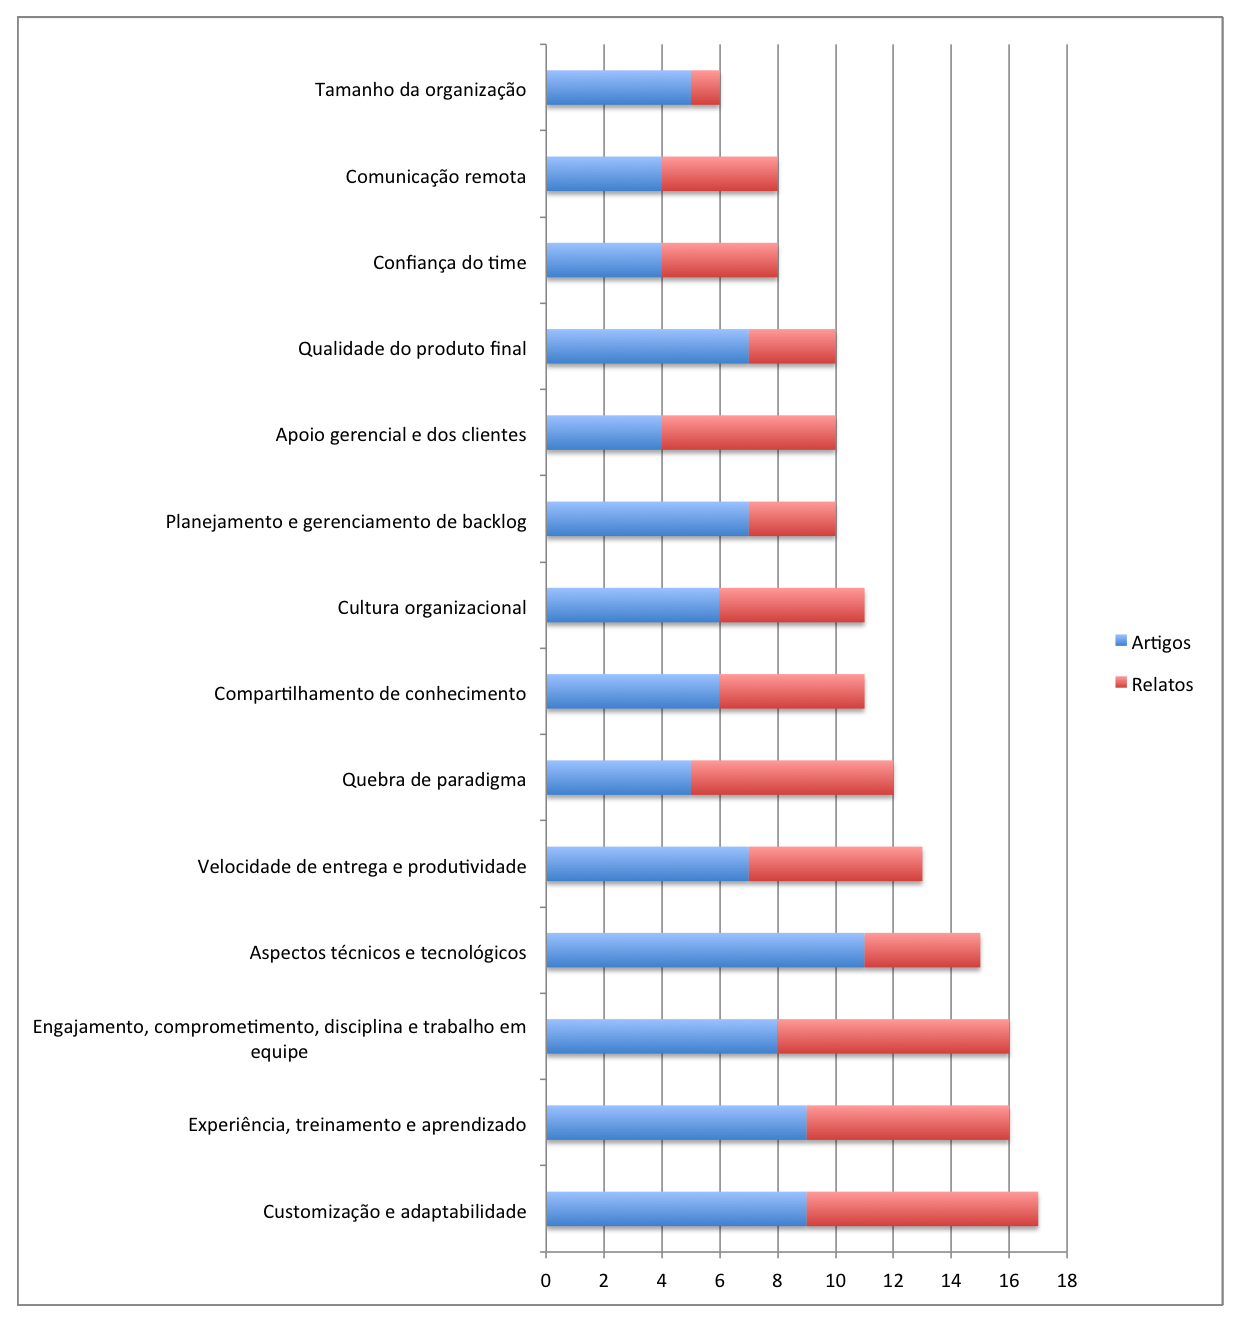
\includegraphics[width=\textwidth]{capitulos/las/figuras/categorias.eps}}
	\caption{Gráfico que contabiliza a quantidade de trabalhos que referenciam cada categoria de lições aprendidas}
	\label{fig:categorias}
\end{figure}

\section{Lições aprendidas}

\subsection{Experiência, treinamento e aprendizado}

\begin{table}[H]
	\centering
	\begin{tabularx}{\linewidth}{ | X | p{5cm} | } \hline \textbf{Lições aprendidas} & \textbf{Referências} \\ \hline
		É muito difícil aventurar-se em ágil sem um Agile Coach & \cite{Hajjdiab2011}, \cite{Block2011}, \cite{Adobe2012}, \cite{Cisco2011}, \cite{Lapham2012}, \cite{Eunha2012}, \cite{Claudia2013}, \cite{Stefano2013}, \cite{Rodrigues2013}, \cite{Bastos2013}, \cite{Maciel2013}, \cite{Karaj2013} \\ \hline
		Vivenciar um projeto-piloto é uma prática muito eficiente para se adquirir experiência & \cite{Hajjdiab2011}, \cite{Cisco2011}, \cite{Rodrigues2013}, \cite{Maciel2013} \\ \hline
		É preciso prática, não apenas estudo & \cite{Hajjdiab2011}, \cite{Asnawi2012}, \cite{Claudia2013}, \cite{Piegas2012}, \cite{Vieira2013} \\ \hline
		Trabalhar com equipes não-agéis pode atrapalhar o andamento do projeto & \cite{Adobe2012}, \cite{Maciel2013} \\ \hline
	\end{tabularx}
\end{table}

Por muitos anos empresas de desenvolvimento de software adotaram o modelo cascata como forma de gerenciamento de projetos. O Manifesto Ágil \cite{agileManifesto}, ocorrido em 2001, modificou completamente a maneira de lidar com esse tipo de atividade.

Mudar bruscamente nunca é simples. Para que esta transição não seja tão dolorosa, uma tática muito popular entre as empresas é a contratação de um profissional experiente para servir como guia e treinar toda a equipe. Segundo \cite{Hajjdiab2011}, este papel é essencial durante o processo de adoção ágil em qualquer organização. Outra maneira de se adquirir experiência de forma rápida e eficaz é através de um projeto-piloto. \cite{Cisco2011} utilizou esta abordagem para entender melhor como a empresa funcionava e atacar nos pontos mais críticos.

Alguns pontos negativos também foram levantados nos trabalhos analisados. Para \cite{Piegas2012}, é preciso aprender com os próprios erros, não apenas realizar treinamentos. E, de acordo com \cite{Adobe2012} e \cite{Maciel2013}, trabalhar com stakeholders que não são ágeis pode afetar negativamente o desempenho do time ágil (que trabalha em um ambiente menos burocrático e com um ciclo de feedback bem mais curto).

\begin{figure}[h]
	\centering
	\captionsetup{justification=centering}
	\makebox[\textwidth]{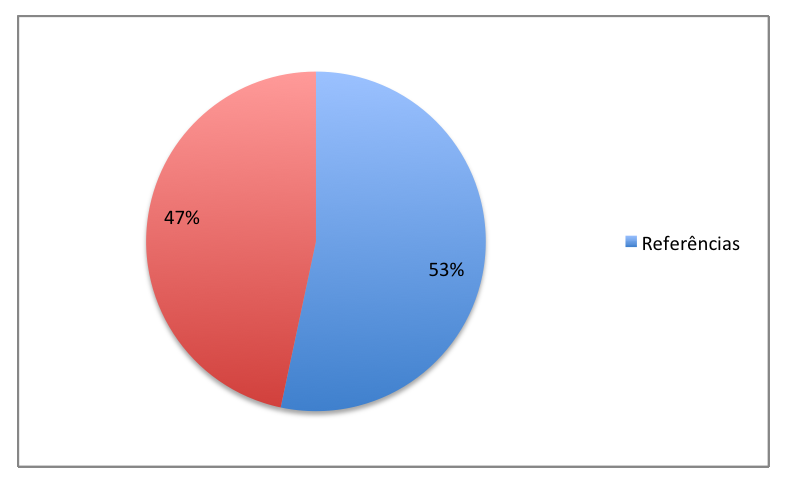
\includegraphics[width=\textwidth]{capitulos/las/figuras/exp.eps}}
	\caption{Gráfico com o percentual de trabalhos que referenciam lições aprendidas da categoria ``Experiência, treinamento e aprendizado"}
	\label{fig:exp}
\end{figure}

\subsection{Planejamento e gerenciamento de backlog}

\begin{table}[H]
	\centering
	\begin{tabularx}{\linewidth}{ | X | p{5cm} | } \hline \textbf{Lições aprendidas} & \textbf{Referências} \\ \hline
		Planejar apenas quando necessário & \cite{Hajjdiab2011}, \cite{Fitzgerald2013}, \cite{Piegas2012}, \cite{Hui2013}, \cite{Parzinello2012} \\ \hline
		O processo de adoção em si precisa ser bem planejado & \cite{Hajjdiab2011} \\ \hline
		Priorizar o backlog é uma tarefa complicada para times inexperientes & \cite{Block2011} \\ \hline
		É difícil lidar com o aumento de escopo & \cite{Block2011} \\ \hline
		É preciso aprender a quebrar o backlog da forma correta & \cite{Adobe2012}, \cite{Hui2013}, \cite{Parzinello2012} \\ \hline
		A coleta e gerência de requisitos ocorre de forma bem diferente do habitual & \cite{Bustard2013}, \cite{Korhonen2010}, \cite{Claudia2013}, \cite{Piegas2012}, \cite{Hui2013} \\ \hline
	\end{tabularx}
\end{table}

Desenvolver de forma iterativa e incremental gera um grande impacto na forma de gerenciamento de projetos ágeis. Não é necessário planejar todas as etapas do processo, é difícil prever situações e cenários muito distantes. Planejar apenas o necessário, quando necessário, é um grande desafio para muitas empresas. O paper \cite{Fitzgerald2013} relata que teve que lidar com muitos problemas relacionados à granularidade no planejamento que Ágil propõe.

Todavia, não podemos confundir o processo planejamento utilizado em projetos ágeis e o planejamento para se adotar ágil. Dado que esta é uma grande mudança de paradigma, é preciso ter cautela. \cite{Hajjdiab2011} aconselha que este processo deve ser bem planejado e que aconteça de forma gradual.

Outro ponto considerado desafiador por muitas organizações é o gerenciamento de backlog. O artigo \cite{Block2011} relata que passou por dificuldades ao tentar priorizá-lo e impedir que ele crescesse além do comportado pela equipe. Ainda com relação ao backlog, \cite{Adobe2012} lembra que um dos princípios primários do desenvolvimento ágil de software é o foco na entrega de pequenos incrementos de valor. Isto pode até parecer simples à primeira impressão, porém dividir todo um conjunto de requisitos de um projeto em pequenas fatias independentes entre si e que agregam valor ao cliente não é algo trivial.

\subsection{Apoio gerencial e dos clientes}

\begin{table}[H]
	\centering
	\begin{tabularx}{\linewidth}{ | X | p{5cm} | } \hline \textbf{Lições aprendidas} & \textbf{Referências} \\ \hline
		Pressão por parte do alto escalão da empresa afeta negativamente no andamento do processo de adoção ágil & \cite{Hajjdiab2011}, \cite{Cisco2011}, \cite{Claudia2013}, \cite{Parzinello2012}, \cite{Stefano2013}, \cite{Bastos2013}, \cite{Maciel2013}, \cite{Srinath2012} \\ \hline
		O apoio do cliente é de suma importância para o sucesso do projeto & \cite{Arikpo2011}, \cite{Claudia2013}, \cite{Parzinello2012}, \cite{Stefano2013}, \cite{Maciel2013} \\ \hline
		É muito difícil contornar uma situação quando o cliente pressiona o tima para que se adote práticas waterfall & \cite{Claudia2013}, \cite{Piegas2012}, \cite{Srinath2012} \\ \hline
		É preciso ter liberdade ao se adotar ágil & \cite{Piegas2012}, \cite{Stefano2013}, \cite{Maciel2013} \\ \hline
	\end{tabularx}
\end{table}

Houve uma unanimidade quanto a este ponto. É preferível que todos os envolvidos em projetos de desenvolvimento de software que utilizam alguma metodologia ágil estejam alinhados com o processo. O apoio da gerência e dos clientes é fundamental para o bom desempenho da equipe.

Mais precisamente, em muitos casos, apenas o apoio não é o suficiente. É preciso ter liberdade para se adotar ágil de forma bem sucedida. Muitos materiais \cite{Piegas2012,Stefano2013,Maciel2013} relataram ter tido problemas com esse nível de alinhamento com os princípios ágeis de liberdade e auto-organização.

\subsection{Customização e adaptabilidade}

\begin{table}[H]
	\centering
	\begin{tabularx}{\linewidth}{ | X | p{5cm} | } \hline \textbf{Lições aprendidas} & \textbf{Referências} \\ \hline
		Ágil é customizável, não existem regras no seu processo de adoção & \cite{Hajjdiab2011}, \cite{Piegas2012}, \cite{Hui2013} \\ \hline
		Dar suporte para adaptabilidade é um problema não-trivial & \cite{Block2011}, \cite{Asnawi2012}, \cite{Fitzgerald2013}, \cite{Bustard2013}, \cite{Microsoft2013}, \cite{Lapham2012}, \cite{Claudia2013}, \cite{Nokia2013}, \cite{Rodrigues2013}, \cite{Bastos2013}, \cite{Maciel2013}, \cite{Hui2013}, \cite{Ahmed2008}, \cite{Sahota2012} \\ \hline
		Dificuldades na implantação de mudanças necessárias & \cite{Vieira2013}, \cite{Bastos2013}, \cite{Maciel2013}, \cite{Hui2013}, \cite{Sahota2012} \\ \hline
	\end{tabularx}
\end{table}

Um dos principais pilares do desenvolvimento ágil é encarar mudanças como bem-vindas. Todavia, atingir um nível de maturidade de tal forma que isto ocorra naturalmente é algo para se orgulhar. Muitos trabalhos relataram problemas para dar suporte a esta adaptabilidade. Em muitas situações, times encontram dificuldades para implantar as mudanças necessárias para obter-se um melhor resultado final em seus projetos. Um exemplo claro deste fator é o demonstrado por \cite{Fitzgerald2013}. Segundo seus autores, ambientes regulados e métodos ágeis são frequentemente vistos como fundamentalmente incompatíveis, o que causa uma série de problemas deste gênero.

Outro ponto relevante levantado por alguns trabalhos é o quanto ágil pode ser customizável. Não exite um conjunto pré-definido de regras que devem ser seguidas à risca por aqueles que querem ser ágeis. Ágil é flexível. Segundo \cite{Hajjdiab2011}, um dos principais benefícios do desenvolvimento ágil é a sua capacidade de ser personalizado baseado na cultura e no ambiente da organização que o está adotando.

\subsection{Confiança do time}

\begin{table}[H]
	\centering
	\begin{tabularx}{\linewidth}{ | X | p{5cm} | } \hline \textbf{Lições aprendidas} & \textbf{Referências} \\ \hline
		Entregar mais e entregar valor  ajuda a manter o time confiante & \cite{Block2011}, \cite{Asnawi2012}, \cite{Parzinello2012} \\ \hline
		Utilizar métodos ágeis ajuda a manter elevada a moral do time & \cite{Asnawi2012}, \cite{Claudia2013}, \cite{Nokia2013}, \cite{Ahmed2008} \\ \hline
		A manutenção da confiança das partes envolvidas mostrou-se comprometida com o uso de metodologias ágeis & \cite{Nokia2013}, \cite{Piegas2012}, \cite{Bastos2013} \\ \hline
	\end{tabularx}
\end{table}

Antes de analisar este ponto, é preciso ter em mente que Ágil não é (nem nunca quis ser) a solução dos problemas causados por processos orientados a planejamento. Não existe bala de prata quanto o assunto é desenvolvimento de software \cite{Piegas2012,Microsoft2013}.

Houve uma grande divergência com relação ao impacto causado por Ágil na confiança dos envolvidos. Enquanto vários trabalhos apontaram que o uso de métodos ágeis contribui com a manutenção da moral elevada do time, outros apontaram exatamente o oposto.

De acordo com \cite{Asnawi2012}, o fato de Ágil proporcionar uma maior frequência de entregas de pedaços de software que agregam valor ao cliente torna o desenvolvimento do projeto mais prazeroso, menos estressante.

Em contrapartida, o relato \cite{Nokia2013} afirma que, em certos casos, é desmotivador trabalhar em um cenário onde não há uma visão clara do que está por vir, um claro desalinhamento com princípios ágeis.

\subsection{Engajamento, comprometimento, disciplina e trabalho em equipe}

\begin{table}[H]
	\centering
	\begin{tabularx}{\linewidth}{ | X | p{5cm} | } \hline \textbf{Lições aprendidas} & \textbf{Referências} \\ \hline
		É difícil encontrar pessoas que trabalham bem em equipe & \cite{Block2011} \\ \hline
		É muito importante ter o PO próximo ou, se possível, como membro ativo do time, envolvido em todas as etapas do processo & \cite{Block2011}, \cite{Asnawi2012}, \cite{Lapham2012}, \cite{Microsoft2013}, \cite{Claudia2013}, \cite{Piegas2012}, \cite{Parzinello2012}, \cite{Stefano2013}, \cite{Rodrigues2013}, \cite{Maciel2013} \\ \hline
		Falta de ownership no projeto & \cite{Block2011}, \cite{Nokia2013}, \cite{Queiroz2013} \\ \hline
		O envolvimento dos desenvolvedores dentro do processo é extremamente importante & \cite{Asnawi2012}, \cite{Adobe2012}, \cite{Fitzgerald2013}, \cite{Lapham2012}, \cite{Microsoft2013}, \cite{Claudia2013}, \cite{Stefano2013}, \cite{Bastos2013}, \cite{Maciel2013}, \cite{Ahmed2008} \\ \hline
		Para projetos ágeis serem bem sucedidos, é preciso disciplina & \cite{Parzinello2012} \\ \hline
	\end{tabularx}
\end{table}

\nomenclature{PO}{Product Owner}%

Para que a construção e entrega de um software sejam bem sucedidas, é preciso esforço de diversas pessoas: desenvolvedores, analistas de qualidade, analistas de negócio, product owners, etc. Ficou bem claro que, para as empresas de desenvolvimento de software analisadas, todos os stakeholders precisam estar fortemente envolvidos em todas as etapas do processo de construção produto. Contudo, um desafio visualizado através dos artigos e relatos foi o de manter o PO engajado. Um exemplo citado por \cite{Block2011} é a dificuldade em manter o cliente próximo para que ele definisse novas funcionalidades e priorizasse o backlog. Situações como esta podem prejudicar consideravelmente o resultado final do projeto, causando frustração para ambos os lados.

Outro ponto pouco citado, porém relevante, é a questão da disciplina em projetos ágeis. Dado que, na teoria, deveríamos ter um ambiente menos controlado e com times auto-organizáveis, esta é uma característica que precisa surgir naturalmente, visto que não existe um plano detalhado a ser seguido. \cite{Parzinello2012} afirma que não se deve culpar o SCRUM (umas das metodologias ágeis mais populares) por sua falta de disciplina.

\subsection{Aspectos técnicos e tecnológicos}

\begin{table}[H]
	\centering
	\begin{tabularx}{\linewidth}{ | X | p{5cm} | } \hline \textbf{Lições aprendidas} & \textbf{Referências} \\ \hline
		Utilizar ágil em um projeto com código legado mostrou-se desafiador & \cite{Block2011} \\ \hline
		Integração contínua, automação de build e testes automatizados promovem ganhos muito vantajosos & \cite{Block2011}, \cite{Microsoft2013}, \cite{Korhonen2010}, \cite{Cisco2011}, \cite{Lapham2012}, \cite{Eunha2012} \\ \hline
		É necessário o suporte de boas ferramentas & \cite{Fitzgerald2013}, \cite{Microsoft2013}, \cite{Arikpo2011} \\ \hline
		A atividade de design arquitetural mostrou-se desafiadora & \cite{Bustard2013}, \cite{Radha2012}, \cite{Piegas2012} \\ \hline
		Ágil promove uma melhor manutenibilidade do código & \cite{Bustard2013} \\ \hline
		Infra-estruturas virtualizadas proporcionam a flexibilidade necessária para muitos projetos ágeis & \cite{Radha2012} \\ \hline
		Ágil promove uma pior manutenibilidade do código & \cite{Nokia2013}, \cite{Queiroz2013} \\ \hline
		Em certos casos há resistência por parte do cliente para utilizar o produto construído & \cite{Stefano2013} \\ \hline
	\end{tabularx}
\end{table}

Aspectos técnicos são muito peculiares, variam de projeto para projeto. Por conta disto, várias lições aprendidas referentes a estes aspectos foram coletadas. Todavia, um padrão analisado é que muitas fontes fazem alusão a uma prática relativamente comum em projetos ágeis: a implantação de um servidor de integração contínua. Pode-se usufruir de muitos benefícios a partir desta prática, como, por exemplo, a automação de testes e deploy automático de código. Para \cite{Block2011}, estas mudanças técnicas tiveram um papel fundamental no nível de sucesso que puderam conquistar com práticas ágeis.

Não planejar todos os detalhes de um projeto antes do seu início causa uma série de impactos no seu fluxo de atividades. Uma área bastante afetada por esta característica de Ágil é o design arquitetural. Diversos materiais afirmaram ter tido problemas com isto. Segundo \cite{Bustard2013}, algumas empresas consideraram Ágil um retrocesso neste aspecto.

A manutenibilidade de código foi o ponto polêmico desta categoria. \cite{Nokia2013} relatou passar por dificuldades em gerenciar muitas pessoas modificando o mesmo código simultaneamente, enquanto \cite{Bustard2013} mostra que diversas empresas comentaram que a melhoria na qualidade e manutenibilidade do código foi um dos principais ganhos com o uso de metodologias ágeis.

\subsection{Compartilhamento de conhecimento}

\begin{table}[H]
	\centering
	\begin{tabularx}{\linewidth}{ | X | p{5cm} | } \hline \textbf{Lições aprendidas} & \textbf{Referências} \\ \hline
		Compartilhar conhecimento e experiências é crucial para o sucesso de projetos ágeis & \cite{Asnawi2012}, \cite{Cisco2011}, \cite{Lapham2012}, \cite{Radha2012}, \cite{Eunha2012}, \cite{Valerio2013}, \cite{Vieira2013}, \cite{Queiroz2013}, \cite{Bastos2013}, \cite{Maciel2013} \\ \hline
		O ambiente com uma cultura ágil favorece o compartilhamento de conhecimento & \cite{Ericsson2013} \\ \hline
	\end{tabularx}
\end{table}

Segundo o Manifesto Ágil \cite{agileManifesto}, indivíduos e interações entre eles devem ser mais valorizados que processos e ferramentas. Outro ponto citado pelo Manifesto é que o método mais eficiente e eficaz de transmitir informações para, e por dentro de um time de desenvolvimento, é através de uma conversa cara a cara. \cite{Ericsson2013} percebeu que Ágil de fato proporciona um ambiente que favorece esta troca de informações, tanto entre projetos como entre pessoas de um mesmo projeto. Muitos trabalhos evidenciaram a importância do compartilhamento de conhecimento pada o sucesso de projetos ágeis, nenhum se opôs a isto.

\subsection{Velocidade de entrega e produtividade}

\begin{table}[H]
	\centering
	\begin{tabularx}{\linewidth}{ | X | p{5cm} | } \hline \textbf{Lições aprendidas} & \textbf{Referências} \\ \hline
		Há um aumento na velocidade/frequência de entrega com ágil & \cite{Adobe2012}, \cite{Fitzgerald2013}, \cite{Microsoft2013}, \cite{Cisco2011}, \cite{Korhonen2010}, \cite{Eunha2012}, \cite{Claudia2013}, \cite{Stefano2013}, \cite{Queiroz2013}, \cite{Maciel2013}, \cite{Hui2013}, \cite{Ahmed2008} \\ \hline
		Defeitos são corrigidos mais rapidamente & \cite{Microsoft2013}, \cite{Korhonen2010} \\ \hline
		A velocidade do time é variável & \cite{Piegas2012} \\ \hline
	\end{tabularx}
\end{table}

A maneira como projetos ágeis são estruturados (iterativos e incrementais) proporciona uma maior quantidade de entregas ao longo do tempo. Este foi um ponto percebido por diversos materiais. No caso de \cite{Fitzgerald2013}, as releases frequentes e a ativa sincronização com  seus clientes fez com que solicitações pudessem ser resolvidas num tempo, em média, menor que cinco semanas, fator que contribuiu para uma maior satisfação do cliente. Segundo a pesquisa feita por \cite{Claudia2013}, aumento na produtividade e capacidade de gerenciamento de mudança de prioridades foram os benefícios mais facilmente percebidos ao se adotar Ágil.

Um outro fator bastante relevante foi apontado por \cite{Microsoft2013,Korhonen2010}. Segundo estes artigos, utilizar Ágil não diminui a quantidade de defeitos encontrados no decorrer do projeto. Contudo, o tempo necessário para a correção dos mesmos diminui drasticamente. Comparando-se o tempo necessário para a resolução de defeitos em projetos ágeis com projetos não-ágeis, cerca de 80\% dos defeitos encontrados demoraram mais a serem resolvidos em projetos não-ágeis \cite{Korhonen2010}.

Outra lição aprendida levantada pela pesquisa foi com relação à variação de velocidade de times ágeis. É natural que, após um certo tempo, time ágeis andem a passos constantes, contudo, de acordo com \cite{Piegas2012}, haver uma variação de velocidade é comum, pois não necessariamente todas as sprints possuem a mesma tonalidade.

\subsection{Qualidade do produto final}

\begin{table}[H]
	\centering
	\begin{tabularx}{\linewidth}{ | X | p{5cm} | } \hline \textbf{Lições aprendidas} & \textbf{Referências} \\ \hline
		A melhoria na qualidade e valor agregado do produto é notória ao se desenvolvê-lo utilizando ágil & \cite{Adobe2012}, \cite{Fitzgerald2013}, \cite{Bustard2013}, \cite{Lapham2012}, \cite{Eunha2012}, \cite{Claudia2013}, \cite{Parzinello2012}, \cite{Maciel2013}, \cite{Ahmed2008} \\ \hline
		Testar a aplicação durante o seu desenvolvimento reduz riscos & \cite{Korhonen2010}, \cite{Lapham2012}, \cite{Eunha2012}, \cite{Parzinello2012}, \cite{Ahmed2008} \\ \hline
	\end{tabularx}
\end{table}

Uma lição aprendida bastante mencionada foi o ganho de qualidade com o uso de metodologias ágeis. Algumas práticas adotas por \cite{Adobe2012} foram fundamentais para a obtenção deste ganho: divisão do trabalho em pequenas fatias que agregam valor ao cliente, definição de critérios de aceitação para cada uma dessas pequenas fatias e criação de times multi-funcionais com experiência em testes e engenharia de software. Este ganho de qualidade não é apenas percebido pelo time, mas também pelo cliente.

O motivo para este ganho de qualidade, para muitos trabalhos, é decorrente da maneira de se testar aplicações em projetos ágeis. Automatizar o processo de testes, além de trazer muita segurança para o processo de desenvolvimento do software, propicia um curto ciclo de feedback.

\subsection{Tamanho da organização}

\begin{table}[H]
	\centering
	\begin{tabularx}{\linewidth}{ | X | p{5cm} | } \hline \textbf{Lições aprendidas} & \textbf{Referências} \\ \hline
		Pequenas empresas conseguem obter benefícios mais facilmente ao adotar ágil & \cite{Bustard2013} \\ \hline
		Escalar ágil para empresas ou projetos maiores é complicado, porém não é impossível & \cite{Microsoft2013}, \cite{Claudia2013}, \cite{Korhonen2010}, \cite{Maciel2013} \\ \hline
		É possível implementar ágil parcialmente & \cite{Ericsson2013} \\ \hline
	\end{tabularx}
\end{table}

O Manifesto Ágil não faz menção a restrições com relação ao tamanho da empresa que se deve ou não adotar ágil. Contudo, alguns trabalhos relataram ter passado por muitas dificuldades devido ao tamanho da empresa.

Para \cite{Bustard2013}, empresas menores e mais horizontais conseguem obter benefícios muito mais facilmente. Vários trabalhadores consultados por \cite{Microsoft2013} apontaram que escalabilidade pode ser um problema ao se tentar praticar Ágil.

\subsection{Quebra de paradigma}

\begin{table}[H]
	\centering
	\begin{tabularx}{\linewidth}{ | X | p{5cm} | } \hline \textbf{Lições aprendidas} & \textbf{Referências} \\ \hline
		É difícil lidar com a quebra de paradigma para a implementação de ágil & \cite{Hajjdiab2011}, \cite{Block2011}, \cite{Korhonen2010}, \cite{Lapham2012}, \cite{Arikpo2011}, \cite{Stefano2013}, \cite{Bastos2013}, \cite{Maciel2013} \\ \hline
		A maneira de gerenciar/implementar os testes de softwares construídos em projeto ágeis é desafiadora & \cite{Korhonen2010} \\ \hline
		Colocar princípios acima de práticas & \cite{Maciel2013}, \cite{Parzinello2012}, \cite{Hui2013}, \cite{Ahmed2008}, \cite{Sahota2012} \\ \hline
	\end{tabularx}
\end{table}

Muitas empresas tentam adotar Ágil com a finalidade de apenas usufruir de seus benefícios, contudo, não param para refletir que são fundamentalmente incompatíveis com muitos princípios, como os exemplos citados por \cite{Lapham2012,Bastos2013}. Fazer com que a alta gerência compreenda que é necessário modificar a essência da organização ao invés de simplesmente adotar um conjunto de práticas é algo bastante desafiador. Muitos dos trabalhos analisados mostraram ter tido problemas com isto. É preciso colocar os princípios acima das práticas \cite{Maciel2013}.

Uma das maiores quebras de paradigma está relacionada ao processo de testes ágeis \cite{Korhonen2010}. Passar a testar a aplicação durante o seu processo de desenvolvimento requer muita disciplina e capacidade técnica de implementação, o que geralmente não era tão essencial.

\subsection{Comunicação remota}

\begin{table}[H]
	\centering
	\begin{tabularx}{\linewidth}{ | X | p{5cm} | } \hline \textbf{Lições aprendidas} & \textbf{Referências} \\ \hline
		Coordernar atividades com times distribuídos é algo bastante desafiador & \cite{Adobe2012}, \cite{Microsoft2013}, \cite{Korhonen2010}, \cite{Radha2012}, \cite{Rodrigues2013}, \cite{Vieira2013}, \cite{Bastos2013}, \cite{Maciel2013} \\ \hline
		Sincronizar board virtual e real não é uma tarefa fácil & \cite{Vieira2013} \\ \hline
		Dificuldade ao trabalhar com equipes externas de testes & \cite{Bastos2013} \\ \hline
	\end{tabularx}
\end{table}

Dividir para conquistar é uma estratégia bastante antiga e que, muitas vezes, também se aplica a Ágil. Entretanto, muitas empresas se mostraram incapazes de gerenciar suas atividades diárias ao utilizar desenvolvimento distribuído de software. Atividades corriqueiras como trabalhar com equipes externas de testes \cite{Bastos2013} e sincronização de boards \cite{Vieira2013} se mostraram problemáticas.

Isto não ocorreu apenas com empresas pequenas e inexperientes. Grandes companhias também passaram por problemas desta natureza. \cite{Adobe2012} relata que, ao adotar uma abordagem distribuída em um de seus projetos, atividades corriqueiras como Sprint Planning, Daily Scrum, Sprint Review e Sprint Retrospective se mostraram desafiadoras.

\subsection{Cultura organizacional}

\begin{table}[H]
	\centering
	\begin{tabularx}{\linewidth}{ | X | p{5cm} | } \hline \textbf{Lições aprendidas} & \textbf{Referências} \\ \hline
		Métodos ágeis e ambiente altamente controlados são, em sua essência, culturalmente incompatíveis & \cite{Fitzgerald2013} \\ \hline
		Empresas que discordam de princípios ágeis tendem a falhar caso tentem implantar tais métodos & \cite{Bustard2013}, \cite{Microsoft2013}, \cite{Claudia2013}, \cite{Nokia2013}, \cite{Sahota2012}, \cite{Maciel2013} \\ \hline
		Tentar influenciar/remodelar a cultura da organização é uma tarefa desafiadora & \cite{Eunha2012}, \cite{Rodrigues2013}, \cite{Bastos2013}, \cite{Sahota2012}, \cite{Srinath2012}, \cite{Maciel2013} \\ \hline
	\end{tabularx}
\end{table}

As lições aprendidas desta categoria foram relativamente semelhantes as da categoria ``Quebra de paradigma", porém com um foco mais voltado para a cultura da organização que está tentando adotar Ágil. Aqui ocorreu uma unanimidade. De acordo com as experiências das empresas cujo material foi analisado, tentar influenciar ou remodelar a cultura da organização não é um processo trivial e, caso seja necessário ser feito e falhe, o risco de falha do projeto é bastante elevado.

É preciso abraçar a cultura Ágil, realmente acreditar em seus princípios.


%Incluindo referências bibliográficas
\bibliographystyle{plain} %define o estilo
\bibliography{./bibliografia/referencias} %busca o arquivo referencias.bib

% Incluindo anexos numerados com letras maiusculas.

%\appendix 
% No arquivo, começar com \chapter{Nome do Anexo}
%\include{posfacios/anexo1}

% Fim do texto
\end{document}
%=======================================================================
